\chapter{Análise Pós-Laboratorial e Resultados}

A fase de análise pós-laboratorial tem como propósito reconciliar o modelo matemático ideal com o comportamento físico do circuito montado em bancada. Esta secção contempla o recálculo das funções de transferência utilizando os valores reais dos componentes aferidos pelo multímetro, a extração das magnitudes experimentais e a avaliação comparativa entre a teoria e a prática.

\section{Recálculo dos Parâmetros Teóricos}

As tolerâncias de fabrico dos resistores e capacitores introduzem desvios na alocação dos polos do sistema. Para isolar o erro instrumental do erro paramétrico, as equações deduzidas na análise teórica foram reavaliadas utilizando as medições reais da Tabela \ref{tab:componentes_medidos}.

\subsection{Circuito 1: Filtro Isolado}
Com $R = 21,841\text{ k}\Omega$ e $C = 103,80\text{ nF}$, a frequência de corte recalculada ($f_{c1\_teo}$) e o ganho estático esperado são:
\begin{equation}
	f_{c1\_teo} = \frac{1}{2\pi \cdot 21841 \cdot 103,80 \times 10^{-9}} \approx 70,21\text{ Hz}
\end{equation}
\begin{equation}
	A_{v1\_teo} = 1\text{ V/V } (0\text{ dB})
\end{equation}

\subsection{Circuito 2: Efeito de Carga}
A introdução de $R_L = 32,314\text{ k}\Omega$ em paralelo com $R = 22,021\text{ k}\Omega$ ($C = 110,90\text{ nF}$) altera a resistência equivalente vista pelo condensador para $R_{eq} = R \parallel R_L \approx 13,096\text{ k}\Omega$. O recálculo resulta em:
\begin{equation}
	f_{c2\_teo} = \frac{1}{2\pi \cdot 13096 \cdot 110,90 \times 10^{-9}} \approx 109,58\text{ Hz}
\end{equation}
\begin{equation}
	A_{v2\_teo} = \frac{32,314\text{k}}{22,021\text{k} + 32,314\text{k}} \approx 0,595\text{ V/V } (\approx -4,51\text{ dB})
\end{equation}

\subsection{Circuito 3: Isolamento com Buffer}
Com $R = 21,757\text{ k}\Omega$ e $C = 106,28\text{ nF}$ (sendo $R_L$ isolada pelo ampop), o circuito regressa à sua dinâmica original:
\begin{equation}
	f_{c3\_teo} = \frac{1}{2\pi \cdot 21757 \cdot 106,28 \times 10^{-9}} \approx 68,83\text{ Hz}
\end{equation}
\begin{equation}
	A_{v3\_teo} = 1\text{ V/V } (0\text{ dB})
\end{equation}

\section{Comparação Direta: Teoria vs. Prática}

A Tabela \ref{tab:comparacao_parametros} evidencia a correspondência entre o modelo matemático ajustado e os resultados extraídos no osciloscópio.

\begin{table}[H]
	\centering
	\caption{Comparação entre os parâmetros teóricos recalculados e as medições práticas.}
	\label{tab:comparacao_parametros}
	\renewcommand{\arraystretch}{1.3}
	\begin{tabular}{ccccccc}
		\hline
		\multirow{2}{*}{\textbf{Circuito}} & \multicolumn{3}{c}{\textbf{Frequência de Corte ($f_c$)}} & \multicolumn{3}{c}{\textbf{Ganho DC ($A_v$) em V/V}} \\ \cline{2-7} 
		& \textbf{Teórico} & \textbf{Medido} & \textbf{Erro (\%)} & \textbf{Teórico} & \textbf{Medido} & \textbf{Erro (\%)} \\ \hline
		\textbf{1 (Sem Carga)} & $70,21\text{ Hz}$ & $67,0\text{ Hz}$ & $4,57\%$ & $1,000$ & $0,971$ & $2,90\%$ \\
		\textbf{2 (Com Carga)} & $109,58\text{ Hz}$ & $121,0\text{ Hz}$ & $10,42\%$ & $0,595$ & $0,403$ & $32,2\%$ \\
		\textbf{3 (Com Buffer)} & $68,83\text{ Hz}$ & $69,0\text{ Hz}$ & $0,24\%$ & $1,000$ & $0,960$ & $4,00\%$ \\ \hline
	\end{tabular}
\end{table}

\textit{Nota analítica:} O Circuito 3 apresentou uma precisão notável (erro de apenas 0,24\% na frequência de corte), provando a robustez do \textit{buffer}. A divergência de ganho no Circuito 2 reflete perdas parasitas na protoboard e, possivelmente, a resistência interna do gerador de sinais atuando em série com o divisor de tensão resistivo.

\section{Estimativa Experimental da Magnitude}

Para preparar a sobreposição gráfica no diagrama de Bode (escala \textit{log-log}), calculou-se a magnitude empírica da função de transferência em cada frequência amostrada, dada pela razão $|H| = V_o / V_i$, bem como o seu equivalente em decibéis ($Mag_{dB} = 20 \log_{10}|H|$).

\begin{table}[H]
	\centering
	\caption{Magnitude experimental calculada para o Circuito 1.}
	\label{tab:mag_c1}
	\renewcommand{\arraystretch}{1.2}
	\begin{tabular}{ccccc}
		\hline
		\textbf{Frequência} & \textbf{Entrada ($V_i$)} & \textbf{Saída ($V_o$)} & \textbf{Magnitude $|H|$ (V/V)} & \textbf{Magnitude (dB)} \\ \hline
		$1,34\text{ Hz}$ & $612,0\text{ mV}$ & $624,0\text{ mV}$ & $1,019$ & $+0,16\text{ dB}$ \\
		$13,40\text{ Hz}$ & $3,812\text{ V}$ & $3,631\text{ V}$ & $0,952$ & $-0,42\text{ dB}$ \\
		$33,50\text{ Hz}$ & $4,740\text{ V}$ & $3,977\text{ V}$ & $0,839$ & $-1,52\text{ dB}$ \\
		$50,25\text{ Hz}$ & $4,857\text{ V}$ & $3,756\text{ V}$ & $0,773$ & $-2,23\text{ dB}$ \\
		$67,00\text{ Hz}$ & $4,852\text{ V}$ & $3,510\text{ V}$ & $0,723$ & $-2,81\text{ dB}$ \\
		$83,75\text{ Hz}$ & $4,987\text{ V}$ & $3,158\text{ V}$ & $0,633$ & $-3,97\text{ dB}$ \\
		$107,20\text{ Hz}$ & $5,000\text{ V}$ & $2,701\text{ V}$ & $0,540$ & $-5,35\text{ dB}$ \\
		$167,50\text{ Hz}$ & $5,000\text{ V}$ & $1,967\text{ V}$ & $0,393$ & $-8,10\text{ dB}$ \\
		$335,00\text{ Hz}$ & $5,035\text{ V}$ & $1,111\text{ V}$ & $0,220$ & $-13,12\text{ dB}$ \\
		$670,00\text{ Hz}$ & $5,038\text{ V}$ & $568,0\text{ mV}$ & $0,112$ & $-18,95\text{ dB}$ \\
		$1340,00\text{ Hz}$ & $5,035\text{ V}$ & $305,0\text{ mV}$ & $0,060$ & $-24,35\text{ dB}$ \\ \hline
	\end{tabular}
\end{table}

\begin{table}[H]
	\centering
	\caption{Magnitude experimental calculada para o Circuito 2.}
	\label{tab:mag_c2}
	\renewcommand{\arraystretch}{1.2}
	\begin{tabular}{ccccc}
		\hline
		\textbf{Frequência} & \textbf{Entrada ($V_i$)} & \textbf{Saída ($V_o$)} & \textbf{Magnitude $|H|$ (V/V)} & \textbf{Magnitude (dB)} \\ \hline
		$2,42\text{ Hz}$ & $1,140\text{ V}$ & $460,0\text{ mV}$ & $0,403$ & $-7,88\text{ dB}$ \\
		$24,20\text{ Hz}$ & $4,660\text{ V}$ & $1,850\text{ V}$ & $0,397$ & $-8,02\text{ dB}$ \\
		$60,50\text{ Hz}$ & $5,030\text{ V}$ & $1,850\text{ V}$ & $0,367$ & $-8,70\text{ dB}$ \\
		$90,75\text{ Hz}$ & $5,070\text{ V}$ & $1,690\text{ V}$ & $0,333$ & $-9,54\text{ dB}$ \\
		$121,00\text{ Hz}$ & $5,100\text{ V}$ & $1,470\text{ V}$ & $0,288$ & $-10,80\text{ dB}$ \\
		$193,60\text{ Hz}$ & $5,110\text{ V}$ & $1,210\text{ V}$ & $0,236$ & $-12,51\text{ dB}$ \\
		$302,50\text{ Hz}$ & $5,110\text{ V}$ & $880,0\text{ mV}$ & $0,172$ & $-15,27\text{ dB}$ \\
		$605,00\text{ Hz}$ & $5,110\text{ V}$ & $450,0\text{ mV}$ & $0,088$ & $-21,10\text{ dB}$ \\
		$1210,00\text{ Hz}$ & $5,110\text{ V}$ & $260,0\text{ mV}$ & $0,050$ & $-25,86\text{ dB}$ \\ \hline
	\end{tabular}
\end{table}

\begin{table}[H]
	\centering
	\caption{Magnitude experimental calculada para o Circuito 3.}
	\label{tab:mag_c3}
	\renewcommand{\arraystretch}{1.2}
	\begin{tabular}{ccccc}
		\hline
		\textbf{Frequência} & \textbf{Entrada ($V_i$)} & \textbf{Saída ($V_o$)} & \textbf{Magnitude $|H|$ (V/V)} & \textbf{Magnitude (dB)} \\ \hline
		$1,38\text{ Hz}$ & $760,0\text{ mV}$ & $760,0\text{ mV}$ & $1,000$ & $0,00\text{ dB}$ \\
		$13,80\text{ Hz}$ & $3,980\text{ V}$ & $3,820\text{ V}$ & $0,959$ & $-0,35\text{ dB}$ \\
		$34,50\text{ Hz}$ & $4,820\text{ V}$ & $4,300\text{ V}$ & $0,892$ & $-1,00\text{ dB}$ \\
		$69,00\text{ Hz}$ & $5,030\text{ V}$ & $3,540\text{ V}$ & $0,703$ & $-3,05\text{ dB}$ \\
		$110,40\text{ Hz}$ & $5,110\text{ V}$ & $2,770\text{ V}$ & $0,542$ & $-5,31\text{ dB}$ \\
		$172,50\text{ Hz}$ & $5,110\text{ V}$ & $2,010\text{ V}$ & $0,393$ & $-8,10\text{ dB}$ \\
		$345,00\text{ Hz}$ & $5,110\text{ V}$ & $1,130\text{ V}$ & $0,221$ & $-13,10\text{ dB}$ \\
		$690,00\text{ Hz}$ & $5,110\text{ V}$ & $640,0\text{ mV}$ & $0,125$ & $-18,04\text{ dB}$ \\
		$1380,00\text{ Hz}$ & $5,110\text{ V}$ & $360,0\text{ mV}$ & $0,070$ & $-23,04\text{ dB}$ \\ \hline
	\end{tabular}
\end{table}
\section{Sobreposição Gráfica: Diagramas de Bode}

Utilizando o \textit{script} base do Maxima, os pontos experimentais (frequência vs. magnitude) das Tabelas \ref{tab:mag_c1}, \ref{tab:mag_c2} e \ref{tab:mag_c3} foram inseridos no plano para verificação visual da conformidade do projeto. As Figuras \ref{fig:bode_exp_1}, \ref{fig:bode_exp_2} e \ref{fig:bode_exp_3} ilustram a sobreposição das curvas teóricas recalculadas com as marcas de medição empírica.

\begin{figure}[H]
	\centering
	\begin{minipage}{0.48\textwidth}
		\centering
		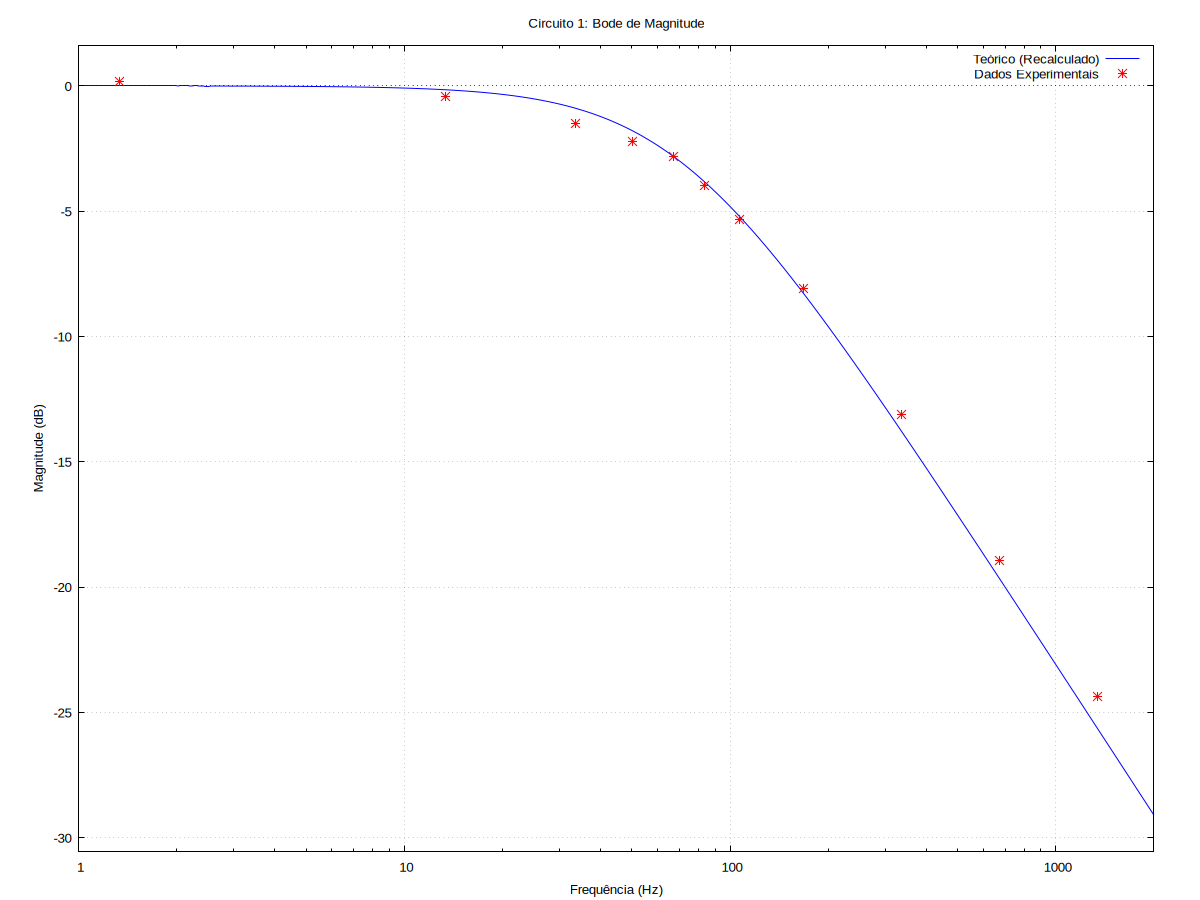
\includegraphics[width=\textwidth]{FIGURAS/bode_exp_1.png}
		\caption{Diagrama de Bode do Circuito 1 com os pontos experimentais.}
		\label{fig:bode_exp_1}
	\end{minipage}\hfill
	\begin{minipage}{0.48\textwidth}
		\centering
		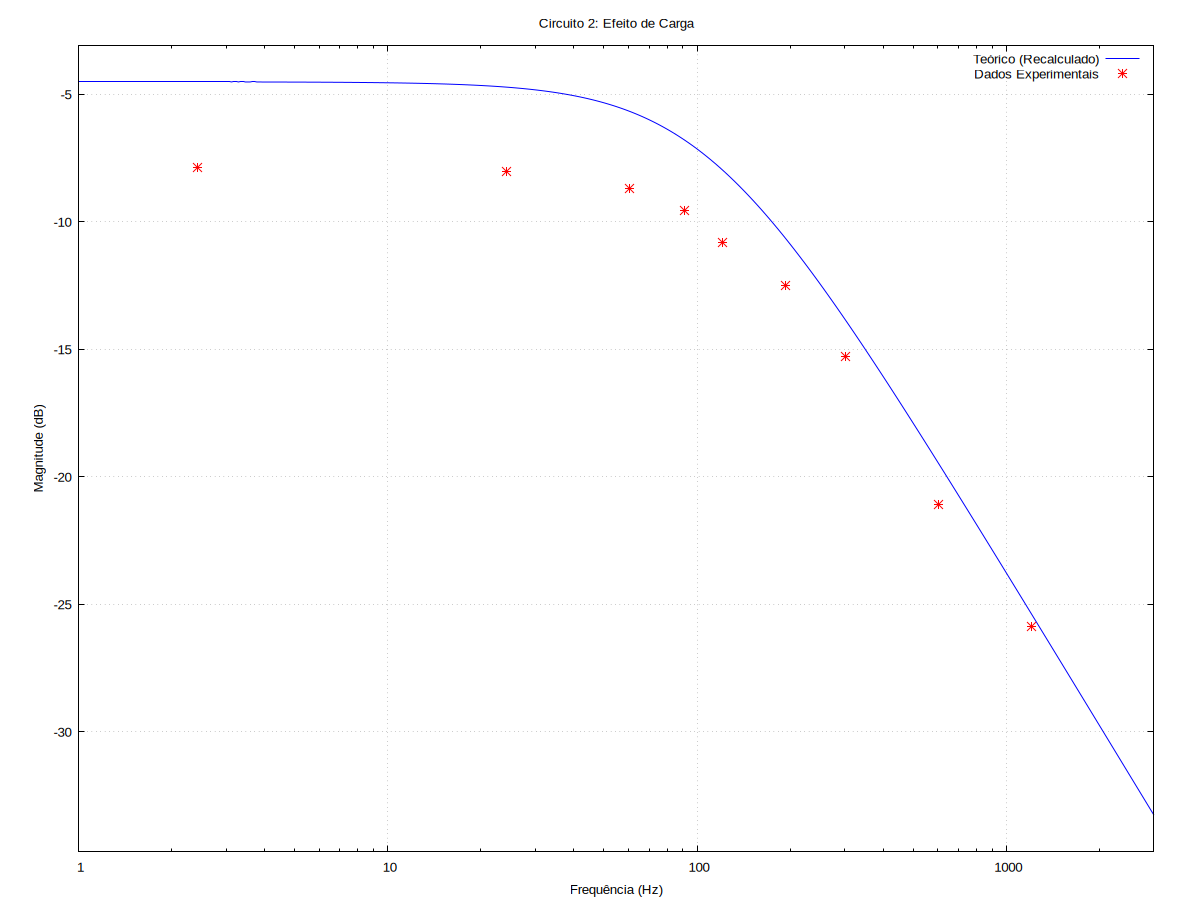
\includegraphics[width=\textwidth]{FIGURAS/bode_exp_2.png}
		\caption{Diagrama de Bode do Circuito 2 evidenciando o Efeito de Carga.}
		\label{fig:bode_exp_2}
	\end{minipage}
\end{figure}

\begin{figure}[H]
	\centering
	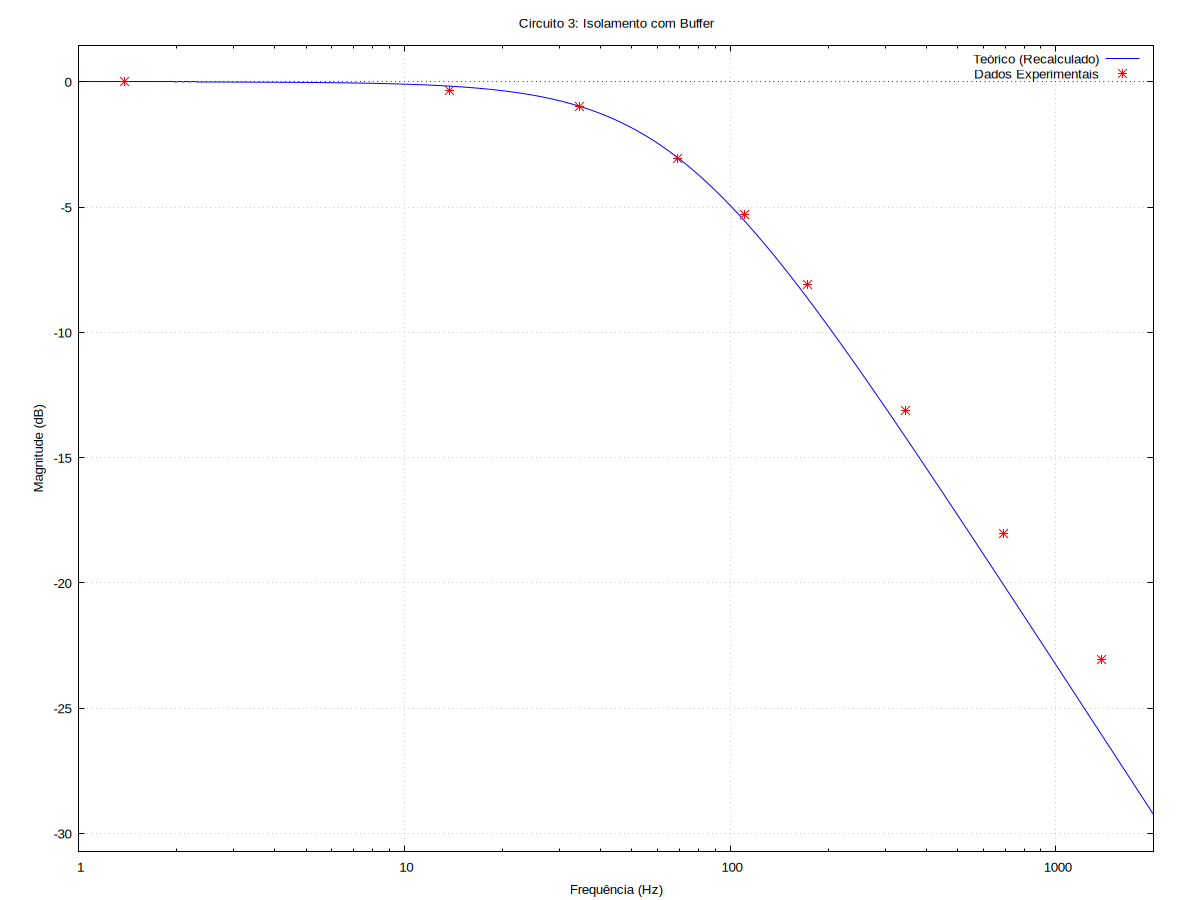
\includegraphics[width=0.55\textwidth]{FIGURAS/bode_exp_3.png}
	\caption{Diagrama de Bode do Circuito 3 comprovando a atuação ideal do \textit{buffer}.}
	\label{fig:bode_exp_3}
\end{figure}